\documentclass[/home/greg/Thesis/main/main.tex]{subfiles}

%\title{Neutron star mechanics in the observers inertial frame}
%\author{}

\begin{document}
\graphicspath{{/home/greg/Neutron_star_modelling/BeamwidthCalculation/img/}}

\newcommand{\ThetaO}{\Theta_{\mathrm{obs}}}
\newcommand{\PhiO}{\Phi_{\mathrm{obs}}}
\newcommand{\sigmaB}{\sigma_{\textrm{beam}}}
\newcommand{\Imax}{I_{\textrm{max}}}
\newcommand{\ThetaT}{\tilde{\Theta}}

\subsubsection{Pulse intensity}

Assuming a fixed magnitude of the magnetic dipole, the pulse intensity will
depend on the orientation of the magnetic dipole to the observer and the beam
geometry. It will be maximal when pointing directly at the observer and
presumably fall off as the angle between the two grows. To model this, we take
an observers position as $(\PhiO, \ThetaO=\iota)$ and then assume the beam geometry
follows Gaussian profile with a single conal emmision. We will assign a maximum
intensity to the beam of $I_0$, then parameterise the beam width by $\sigmaB$.
We can the express the pulse intensity for such a beam geometry as
\begin{equation}
I
(\Theta, \Phi, \iota,  I_{0}, \sigmaB)
=
I_{0} \left(
\exp\left(-\frac{\Delta d^{2}}{2\sigmaB^{2}}\right)+
\right)
\label{eqn: beam intensity}
\end{equation}
The $\Delta d$ quantity
measures the central angle between the observers line of sight and the beam.
We can calculate this spherical distances from the spherical law of cosines
\begin{align}
\Delta d &= \cos^{-1}\left[\cos(\Theta)\cos(\iota) +
                              \sin(\Theta)\sin(\iota)\cos(|\Phi - \PhiO|)\right] \\
\label{eqn: angular sep}
\end{align}

We now have a general expression for the beam intensity from which we can calculate
a maximum observed intensity
\newcommand{\repterm}{\left(\ThetaT - \iota\right)^{2}}
\begin{align}
I_\textrm{max} = I_{0} \exp\left(
    -\frac{\repterm}
          {2\sigmaB}\right)
\label{eqn: Imax}
\end{align}
In figure~\ref{fig: intensity variation} we illustrate the pulse intensity and
maximimal value over a single precessional cycle. We have inentionally chosen
unphysical values to illustrate both the fast pulses and the slow modulation on
the same timescale.

\begin{figure}[htb]
\centering
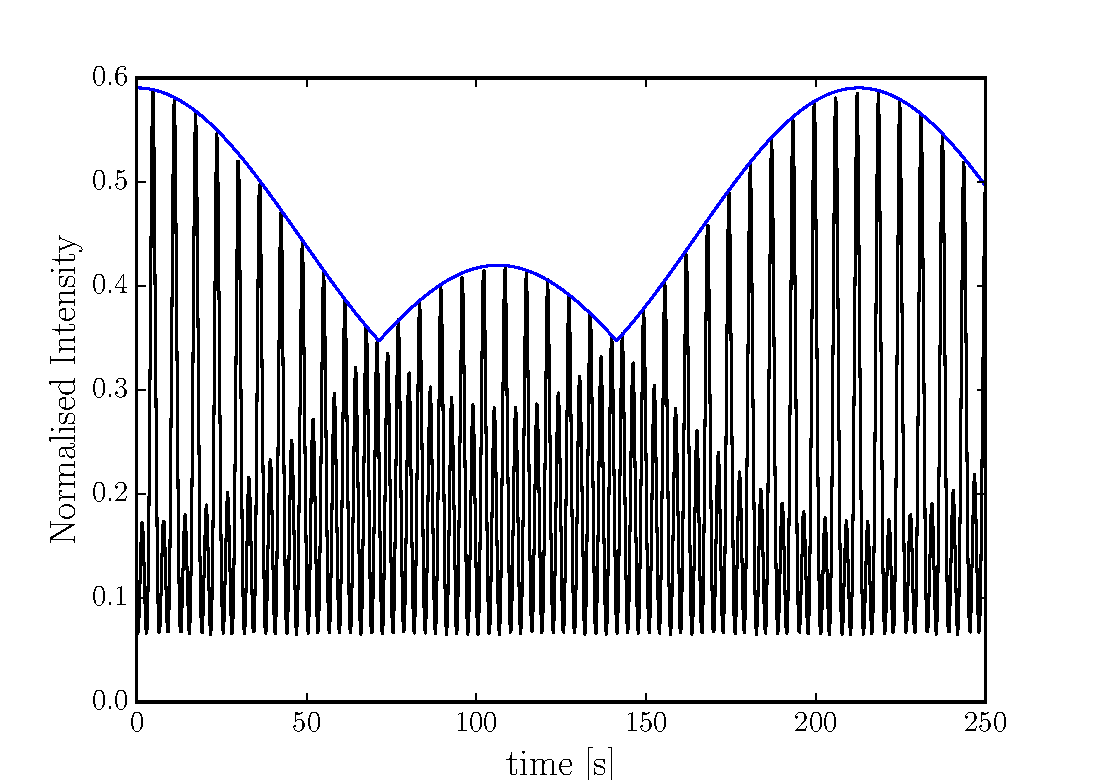
\includegraphics[width=.5\textwidth]{intensity_variation}
\caption{Amplitude variation using a 2D Gaussian emission. In black is the pulse
intensity as given by \eqref{eqn: beam intensity}: this shows each individual
pulse at the fast rotation frequency with the slower modulation due to precession.
In blue we plot the maximum amplitude as described by Eqn.~\eqref{eqn: Imax}.}
\label{fig: intensity variation}
\end{figure}



\FloatBarrier
\subsubsection{Pulse width}
We now need to relate the pulse intensity calculated previously with the quantity
measured by pulsar astronomers: the $W_{10}$ or the width at 10\% of the observed peak
intensity.

Now let us state that $\Theta$ varies on the slow
precession timescale, while $\Phi$ varies on the rapid spin timescale. We are
looking to measure the variations with respect to the slow precession timescale.
The pulse width is measured by the time spent above some fractional amount $p/100$
of the peak measured amplitude; note the convention is to use say 10\% of the peak
value, in our notation then p=10. The condition for when the intensity is greater
than this fraction is
\begin{align}
I > \Imax \frac{p}{100}.
\end{align}
We can substitute into equations~\eqref{eqn: beam intensity} and~\eqref{eqn: Imax}
and rearrange. This gives us an expression for when the inequality is satisfied:
\begin{equation}
\cos(|\Phi|) < \frac{\cos\left(\sqrt{
    (\Theta - \iota)^{2}-2\sigmaB^{2} \ln(\frac{p}{100})}\right)-\cos(\Theta)\cos(\iota)}
    {\sin(\Theta)\sin(\iota)}
\label{eqn: 6737}
\end{equation}
Since we expect $\Theta$ to vary on a much longer timescale than $\Phi$, over
one period in $\Phi$ we can treat $\Theta$, and hence the whole right-hand-side
as a constant. Lets consider a single rotation with the magnetic dipole
starting and ending in the antipodal point to the observers position. Then
$\Phi$ increase beween $-\pi$ and $\pi$ during this rotation. The
time during which this inequality is true, measures the beam width.

In figure \ref{fig: CosineIllustration} an illustration is given of this single
period showing the constant value on the right hand side of \eqref{eqn: 6737} and
the osciallting cosine function. When the cosine is less than this constant
this inequality is satisfied.
\begin{figure}[ht]
\centering
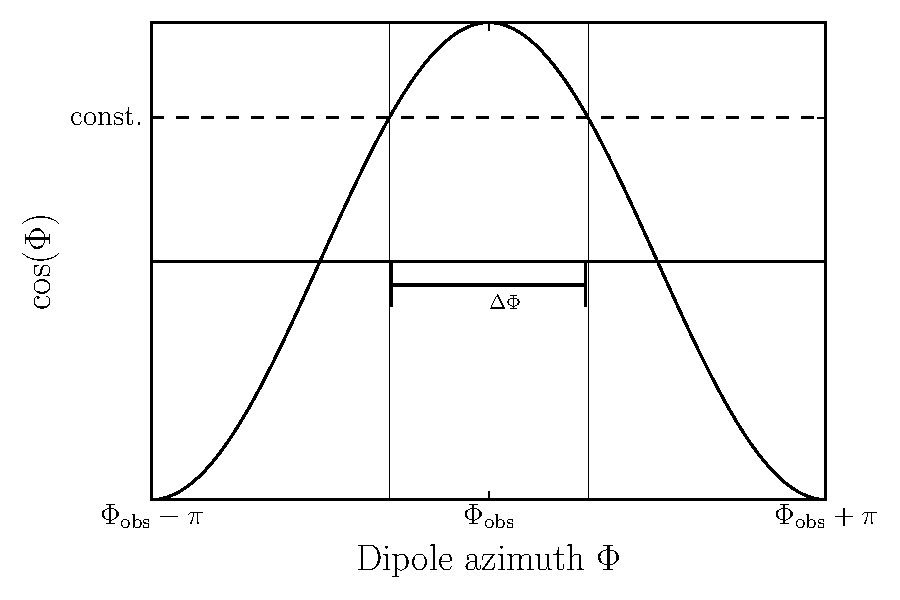
\includegraphics[width=.5\textwidth]{CosineIllustration.pdf}
\caption{Illustration of the inequality in equation \eqref{eqn: 6737} the constant
         value represents the right hand side of this equation. The
         width $\Delta\Phi$ indicates the angular period during which inequality
         is satisfied.}
\label{fig: CosineIllustration}
\end{figure}

We can calculate the beam width measured by observed by first calculating the
angular width $\Delta\Phi$ for which the inequality is not satisified:
\begin{equation}
    \Delta\Phi = 2\cos^{-1}\left(
                \frac{\cos\left(\sqrt{
                    (\Theta - \iota)^{2}-2\sigmaB^{2} \ln(\frac{p}{100})}\right)-\cos(\Theta)\cos(\iota)}
                          {\sin(\Theta)\sin(\iota)}
                      \right)
\end{equation}
Then the angular fraction at which the inequality \emph{is} satisfied is given by
$2\pi - \Delta\Phi$. The beam width is measured in the time spent above the
fraction $f$ of the peak measured amplitude. So we can convert our angular
fraction above into a beam width by

We can now convert this into a pulse width
\begin{align}
    W_p & = P \frac{2\pi - \Delta\Phi}{2\pi} \\
          & = P\left(1 -
               \frac{1}{\pi}\cos^{-1}\left(
                   \frac{\cos\left(\sqrt{\repterm-2\sigmaB^{2} \ln(\frac{p}{100})}\right)
                    - \cos(\Theta)\cos(\iota)}
                          {\sin(\Theta)\sin(\iota)}
                      \right)
                  \right)
\label{eqn: Wp}
\end{align}
where $P$ is the spin period which we have then written in terms of the spin
frequency and $p$ is the percentage of beam width.
the beam width will vary with both the changes in spin-frequency, and with
$\Theta$.

\subsubsection{Illustrations}

In the following figures we demonstrate typical beamwidths alongside the
$\Theta$ behaviour which drives changes in the widths.
\begin{figure}[ht]
\centering
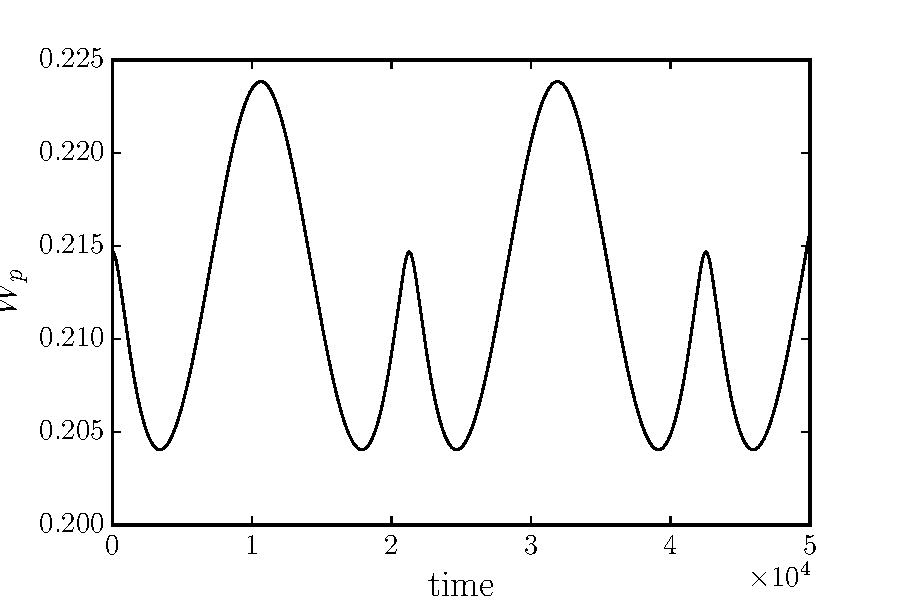
\includegraphics[width=.5\textwidth]{Pulse_width_modulation.pdf}
\caption{The beamwidth and polar angle $\Theta$ of the brightest beam for a pulsar
         with $\Theta < \pi/2$}
\label{fig: Pulse width modulation}
\end{figure}•

\begin{figure}[ht]
\centering
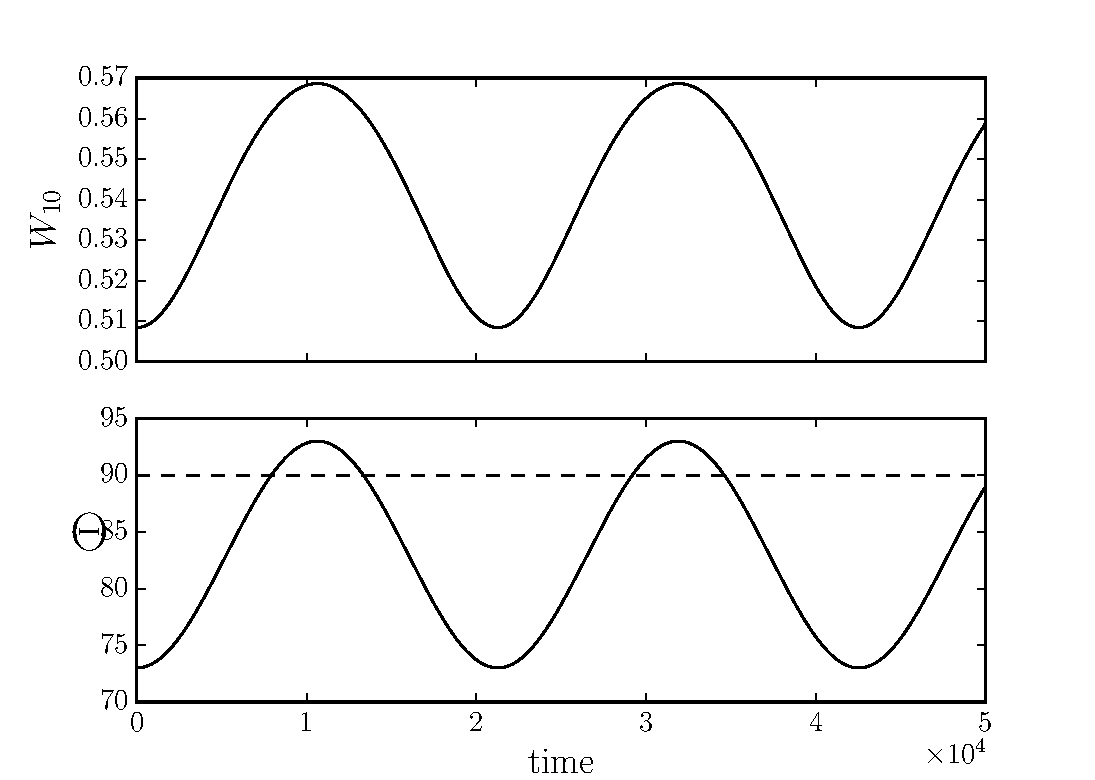
\includegraphics[width=.5\textwidth]{Pulse_width_modulation_chi90.pdf}
\caption{The beamwidth and polar angle $\Theta$ of the brightest beam for a pulsar
         with $\Theta \approx \pi/2$}
\label{fig: Pulse width modulation chi90}
\end{figure}•


\FloatBarrier

\subsubsection{Limits on $\sigmaB$}
So far we have ignored the physical implications of $\sigmaB$, we will now
discuss its limits which will help us to gain some intuition. Inherited
from the our Gaussian beam structure, $\sigmaB$ provides a measure of the
beam width; as such we know that in order to observe a pulse $\sigmaB > 0$, but
the upper limit is somewhat more subtle. The observed pulses arrive in a
'pulse-train' as $\Phi$ increases in Eqn.~\eqref{eqn: beam intensity}.
In order then to measure the $p^{\textrm{rm}}$ percentage of the beamwidth, we
need
\begin{equation}
I_\mathrm{min} < \frac{p}{100}I_\mathrm{max}
\end{equation}
where, for the generalise pulse intensity
\begin{align}
I_\mathrm{max} & = I_{0} \exp\left(-\frac{(\Theta - \iota)^{2}}{2\sigmaB^{2}}\right) \\
I_\mathrm{min} & = I_{0} \exp\left(-\frac{(\Theta + \iota)^{2}}{2\sigmaB^{2}}\right)
\end{align}
Substituting and rearranging for $\sigmaB$ we find that
\begin{equation}
\sigmaB^{2} < \frac{2\Theta\iota}{\log(100/P)}
\end{equation}

\biblio
\end{document}

